\section{Math for Kids - Simple Properties}
\textcite{zhang2019scenario} use a \gls{spa} titled "Math for kids", which generates simple math addition problems and keeps track of a statistic, which includes the number of correctly and incorrectly answered problems as an example. The same application has been implemented and extended in Vue.js and will be used to showcase the capabilities of the interaction diagram and scenario generation application and compare the resulting diagrams to the ones in \parencite{zhang2019scenario}.

\begin{figure}[H]
    \centering
    \begin{subfigure}[t]{0.45\textwidth}
         \centering
         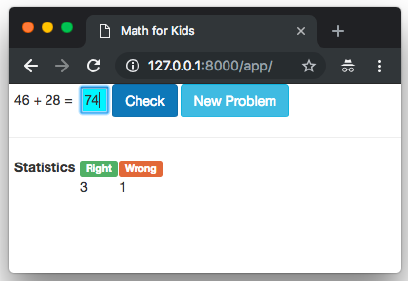
\includegraphics[width=0.45\textwidth]{images/math_for_kids_zhang.png}
         \caption{Math for Kids in AngularJS by \textcite{zhang2019scenario}}
    \end{subfigure}\hfill%
    \begin{subfigure}[t]{0.45\textwidth}
        \centering
        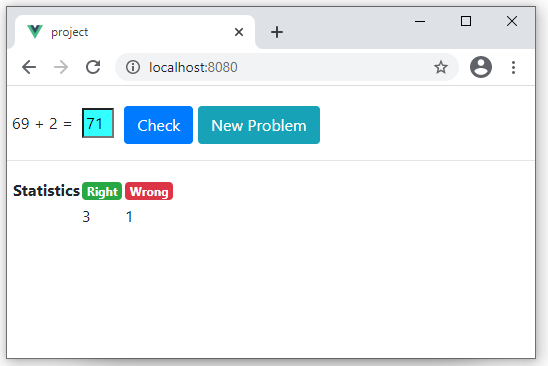
\includegraphics[width=0.45\textwidth]{images/math_for_kids_own.png}
        \caption{Own implementation of Math for Kids in Vue.js}
    \end{subfigure}
\end{figure}

The source code can be found in \code{resources/test-files/test.vue} and also in \ref{appendix:math_kids_basic_source_code}.
\begin{figure}[H]
    \centering
    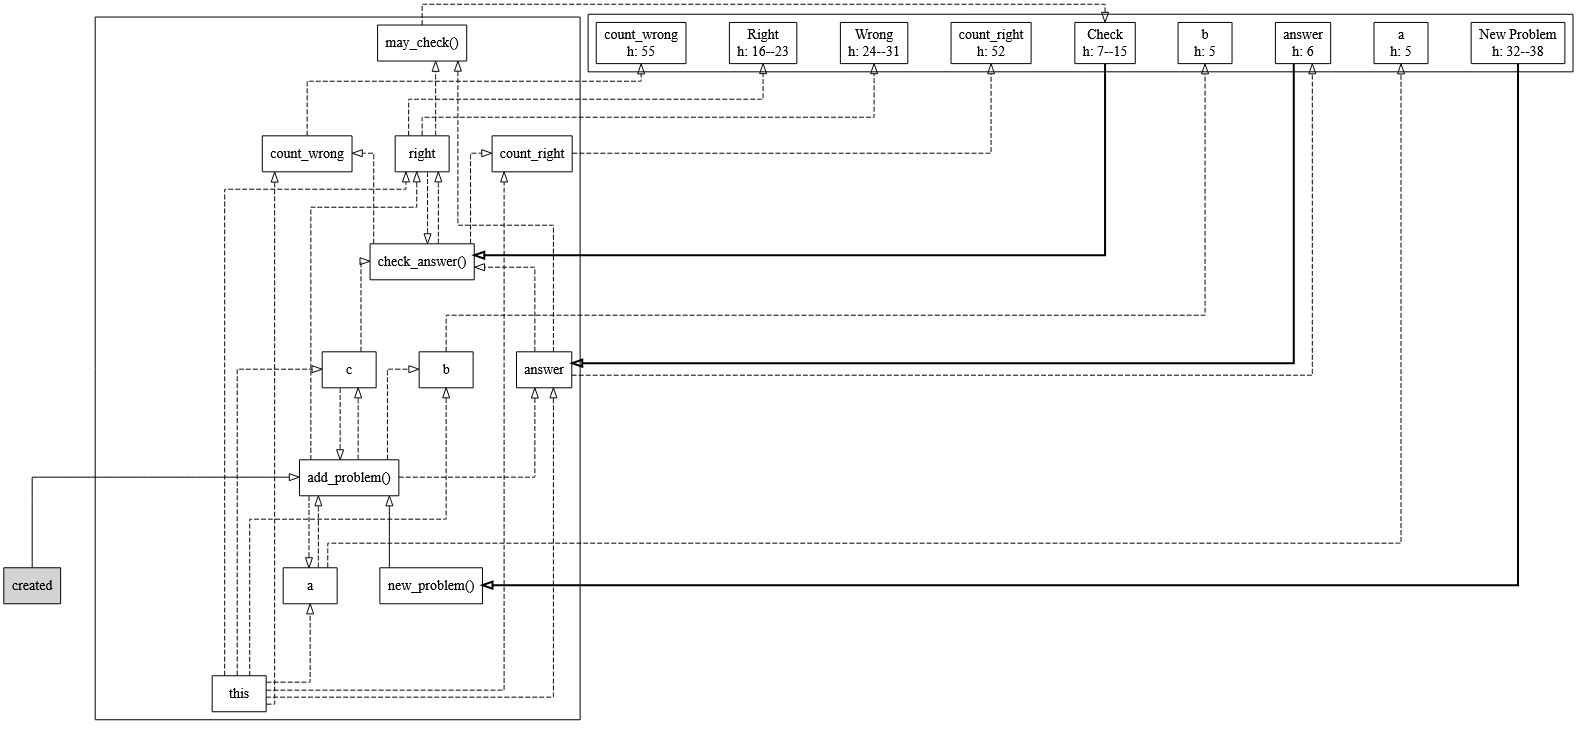
\includegraphics[width=0.9\textwidth]{images/diagram_own_math_kids.png}
     \caption{Math for Kids in Vue.js generated interaction diagram }
     \label{fig:math_for_kids_own_interaction_diagram}
\end{figure}

\begin{figure}[H]
    \centering
    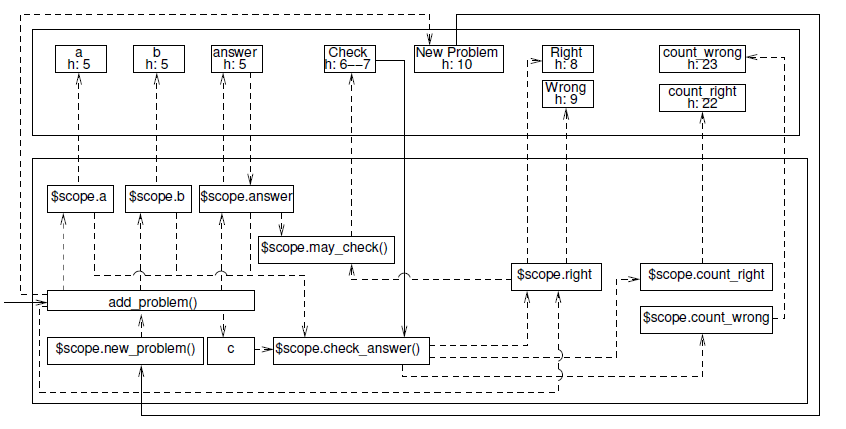
\includegraphics[width=0.9\textwidth]{images/interaction_diagram_zhang.png}
     \caption{Math for Kids in AngularJS interaction diagram by \textcite{zhang2019scenario}}
     \label{fig:math_for_kids_zhang_interaction_diagram}
\end{figure}

When comparing the generated diagram \ref{fig:math_for_kids_own_interaction_diagram} to the original \ref{fig:math_for_kids_zhang_interaction_diagram} by \textcite{zhang2019scenario}  there are some differences.

Due to different modelling there is a \code{this} vertex and connections from it to top level variables, which does not exist in the diagram by \textcite{zhang2019scenario}. In the generated diagram there is an edge of type 'event' between the \code{answer} tag and \code{answer} property. This is due to the difference in two-way bindings representation.

There are two differences between the \code{add_problem} node in the generated diagram and the one by \parencite{zhang2019scenario}.
In \textcite{zhang2019scenario} there is an edge from
the \code{add_problem} method to the \code{New Problem} tag, which is missing in the own generated version. This seems like a mistake in \parencite{zhang2019scenario}, since this edge should not exist.

The other difference is that in \parencite{zhang2019scenario} there is no edges from \code{add_problem} to \code{right} (write relation), however there should be, since
inside \code{add_problem}, \code{this.right = undefined}.

\begin{lstlisting}[language=JavaScriptPlain]
l(created) -> a, b, answer, Check, Right, Wrong
l(answer) -> answer, Check
l(Check) -> Right, Wrong, Check, count_right, count_wrong
l(New Problem) -> a, b, answer, Check, Right, Wrong
\end{lstlisting}

The generated interactions differ for $l(created)$, all other sets are exactly the same as the ones by \textcite{zhang2019scenario} (albeit in different order). This may stem from the fact that the edges of \code{add_problem} to \code{\$scope.right} is missing in \parencite{zhang2019scenario}, however it is later correctly factored in $l(\textrm{New Problem})$.

\textcite{zhang2019scenario} define the initial interaction as \code{l(add_problem() = 
\{a, b\}} 
whereas it should be 
\code{l(add_problem() = \{Check, Right, Wrong, a, b, answer \}} since the answer property is updated based on the diagram. 

One could argue, that the version in \parencite{zhang2019scenario} is correct, since $answer$ is set to $undefined$, which is the same as the initial value of the variable, so it would not trigger an update as part of the \code{init} method. The interaction diagram generator does not perform this check. If \code{add_problem()} were to be called later in the application (when the \code{New Problem} button is clicked) it would indeed set a new value to \code{answer}, which is correctly reflected by \textcite{zhang2019scenario}.


\subsection{Scenarios}
The generated Gherkin scenario templates of up to 4 actions can be seen in \ref{fig:eval_gherkin}. The program outputs the scenarios as plain text to the console, but here they are displayed in a nicer way. The caption of each figure is an example of how a text could be generated based on the template scenario output by the application. Some scenarios seem a bit repetitive, but it is up to \textit{The Three Amigos} \ref{amigos} to decide which templates to discard, since interaction diagrams model what \textit{might} be updated. The fact that everything which might get updated is displayed can also be leveraged in another way - negative criteria can be defined (verify component or tag $X$ did not change).
%TODO play around with subfigure alignment, there be
%https://tex.stackexchange.com/questions/333249/controlling-subfigure-captions-and-subfigure-placement
\begin{figure}[H]
   
    \caption{Gherkin scenario templates and sample human written scenarios based on the templates }
    \label{fig:eval_gherkin}
    \centering
    \begin{subfigure}[t]{0.48\textwidth}
         \centering
         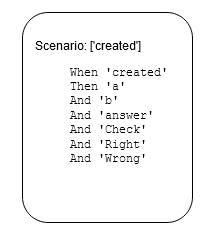
\includegraphics[width=0.48\textwidth]{images/scenarios_1.png}
         \caption{Scenario: initialization. When the application is created, then 'a' and 'b' should show random numbers and 'Check' should be disabled and 'Right' and Wrong should be invisible.}
    \end{subfigure}\hfill%
    \begin{subfigure}[t]{0.48\textwidth}
        \centering
        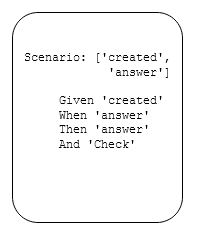
\includegraphics[width=0.48\textwidth]{images/scenarios_2.png}
        \caption{Scenario: typing an answer. Given the application has been created, when I type an answer then 'answer' should display it and 'Check' should be enabled.}
    \end{subfigure}\hfill%
    \begin{subfigure}[t]{0.48\textwidth}
        \centering
        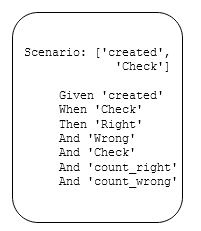
\includegraphics[width=0.48\textwidth]{images/scenarios_3.png}
        \caption{Scenario: clicking on check without typing an answer. Given the application has been created, when I click 'Check' then 'Right' and 'Wrong' should be invisible and 'count\_right' and 'count\_wrong' should have the same values and 'Check' should be disabled. }
   \end{subfigure}\hfill%
   \begin{subfigure}[t]{0.48\textwidth}
    \centering
    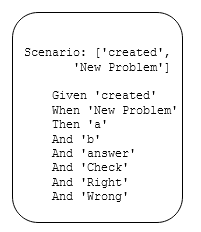
\includegraphics[width=0.48\textwidth]{images/scenarios_4.png}
    \caption{Scenario: obtaining a new problem at application start. Given the application has been created, when I click 'New Problem' then 'a' and 'b' should have random values and 'answer' should be empty and 'Check' should be disabled and 'Right' and 'Wrong' should be invisible.}
\end{subfigure}\hfill%
\end{figure}

\begin{figure}[H]\ContinuedFloat
    \centering

\begin{subfigure}[t]{0.48\textwidth}
    \centering
    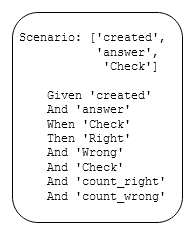
\includegraphics[width=0.48\textwidth]{images/scenarios_5.png}
    \caption{Scenario: checking my answer. Given the application has been created and 'answer' contains my answer, when I click 'Check' then 'Right' should be visible if the answer was right 'Wrong' should be visible if the answer was wrong and 'Check' should be disabled and 'count\_right' should be incremented by one if the answer was right and 'count\_wrong' should be incremented by one if the answer did not change. }
\end{subfigure}\hfill%
\begin{subfigure}[t]{0.48\textwidth}
    \centering
    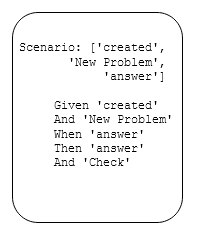
\includegraphics[width=0.48\textwidth]{images/scenarios_6.png}
    \caption{Scenario: typing an answer to a new problem. Given the application has been created and a new problem was obtained, when I type an answer then 'answer' should display it and 'Check' should be enabled.}
\end{subfigure}\hfill%
\begin{subfigure}[t]{0.48\textwidth}
    \centering
    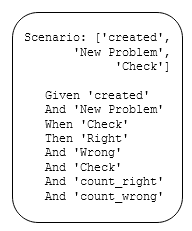
\includegraphics[width=0.48\textwidth]{images/scenarios_7.png}
    \caption{Scenario: requesting a new problem and clicking on check without answering it. Given the application has been created and I requested a new problem, when I click 'Check' then 'Right' and 'Wrong' should be invisible and 'count\_right' and 'count\_wrong' should have the same values and 'Check' should be disabled. }
\end{subfigure}\hfill%
\begin{subfigure}[t]{0.48\textwidth}
    \centering
    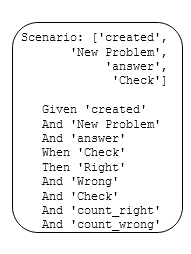
\includegraphics[width=0.48\textwidth]{images/scenarios_8.png}
    \caption{Scenario: requesting a new problem, answering it and checking my answer. Given the application has been created and I requested a new problem and answered it, when I click 'Check' then 'Right' should be visible if the answer was right 'Wrong' should be visible if the answer was wrong and 'Check' should be disabled and 'count\_right' should be incremented by one if the answer was right and 'count\_wrong' should be incremented by one if the answer did not change. }
\end{subfigure}

\end{figure}

\section{Math for Kids Extended - Lists and Computed Properties}
The Math for Kids application has been extended to display a list of past problems and randomly generates either a subtraction or addition problem. It also keeps tracks of statistics separated by problem type and includes and additional accuracy statistic, which is implemented as a computed property. The application can be seen in \ref{fig:eval_image_list_complex} and the full source code can be found it \ref{appendix:math_kids_extended_source_code}
\begin{figure}[H]
    \centering
    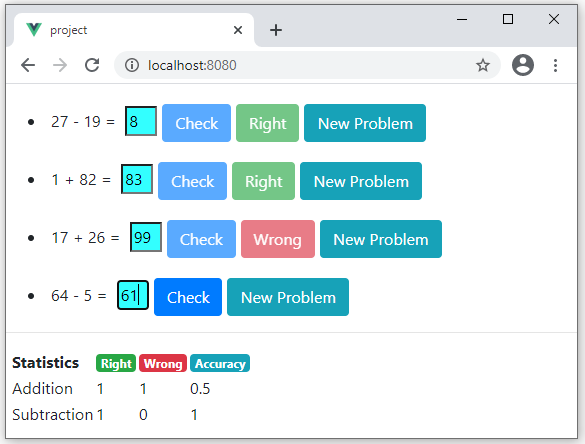
\includegraphics[width=0.6\textwidth]{images/math_for_kids_own_complex.png}
     \caption{Math for Kids in Vue.js including subtraction problems, more precise statistics and display of past problems }
     \label{fig:eval_image_list_complex}
\end{figure}

The resulting interaction diagram  is shown in \ref{fig:diagram_list_complex}. It looks more complex, but it is still possible to focus on specific components and see how they interact with others. 

The two vertices for the computed properties \textit{accuracy\_sub} and \textit{accuracy\_add} correctly directly depend on \textit{count\_right\_sub}, \textit{count\_wrong\_sub} and \textit{count\_right\_add}, \textit{count\_wrong\_add} respectively. By looking at the interactions, one can observe that based on which of the mutually exclusive Check buttons is clicked on, either the substituting or addition related properties are updated. This differentiation is also evident in the generated Gherkin scenario templates. The full list of generated scenario templates of up to 4 actions can be seen in  \ref{appendix:math_kids_extended_scenarios}
\begin{lstlisting}[language=JavaScriptPlain]
    l(problems[i].answer) -> problems[i].answer, Check, Check
    l(Check) -> Right, Wrong, Check, Check, count_right_add, accuracy_add, count_wrong_add
    l(Check) -> Right, Wrong, Check, Check, count_right_sub, accuracy_sub, count_wrong_sub
    l(New Problem) -> problems[i].a, +, -, Check, Check, problems[i].b, problems[i].answer, Right, Wrong
    l(created) -> problems[i].a, +, -, Check, Check, problems[i].b, problems[i].answer, Right, Wrong
    \end{lstlisting}
This example includes a bit of engineering - more realistically there would a single button, which checks inside the bound method which should be updated, however the application would not be able to be differentiate them in this case, since if statements inside methods are not supported. 
\begin{figure}[H]
    \centering
    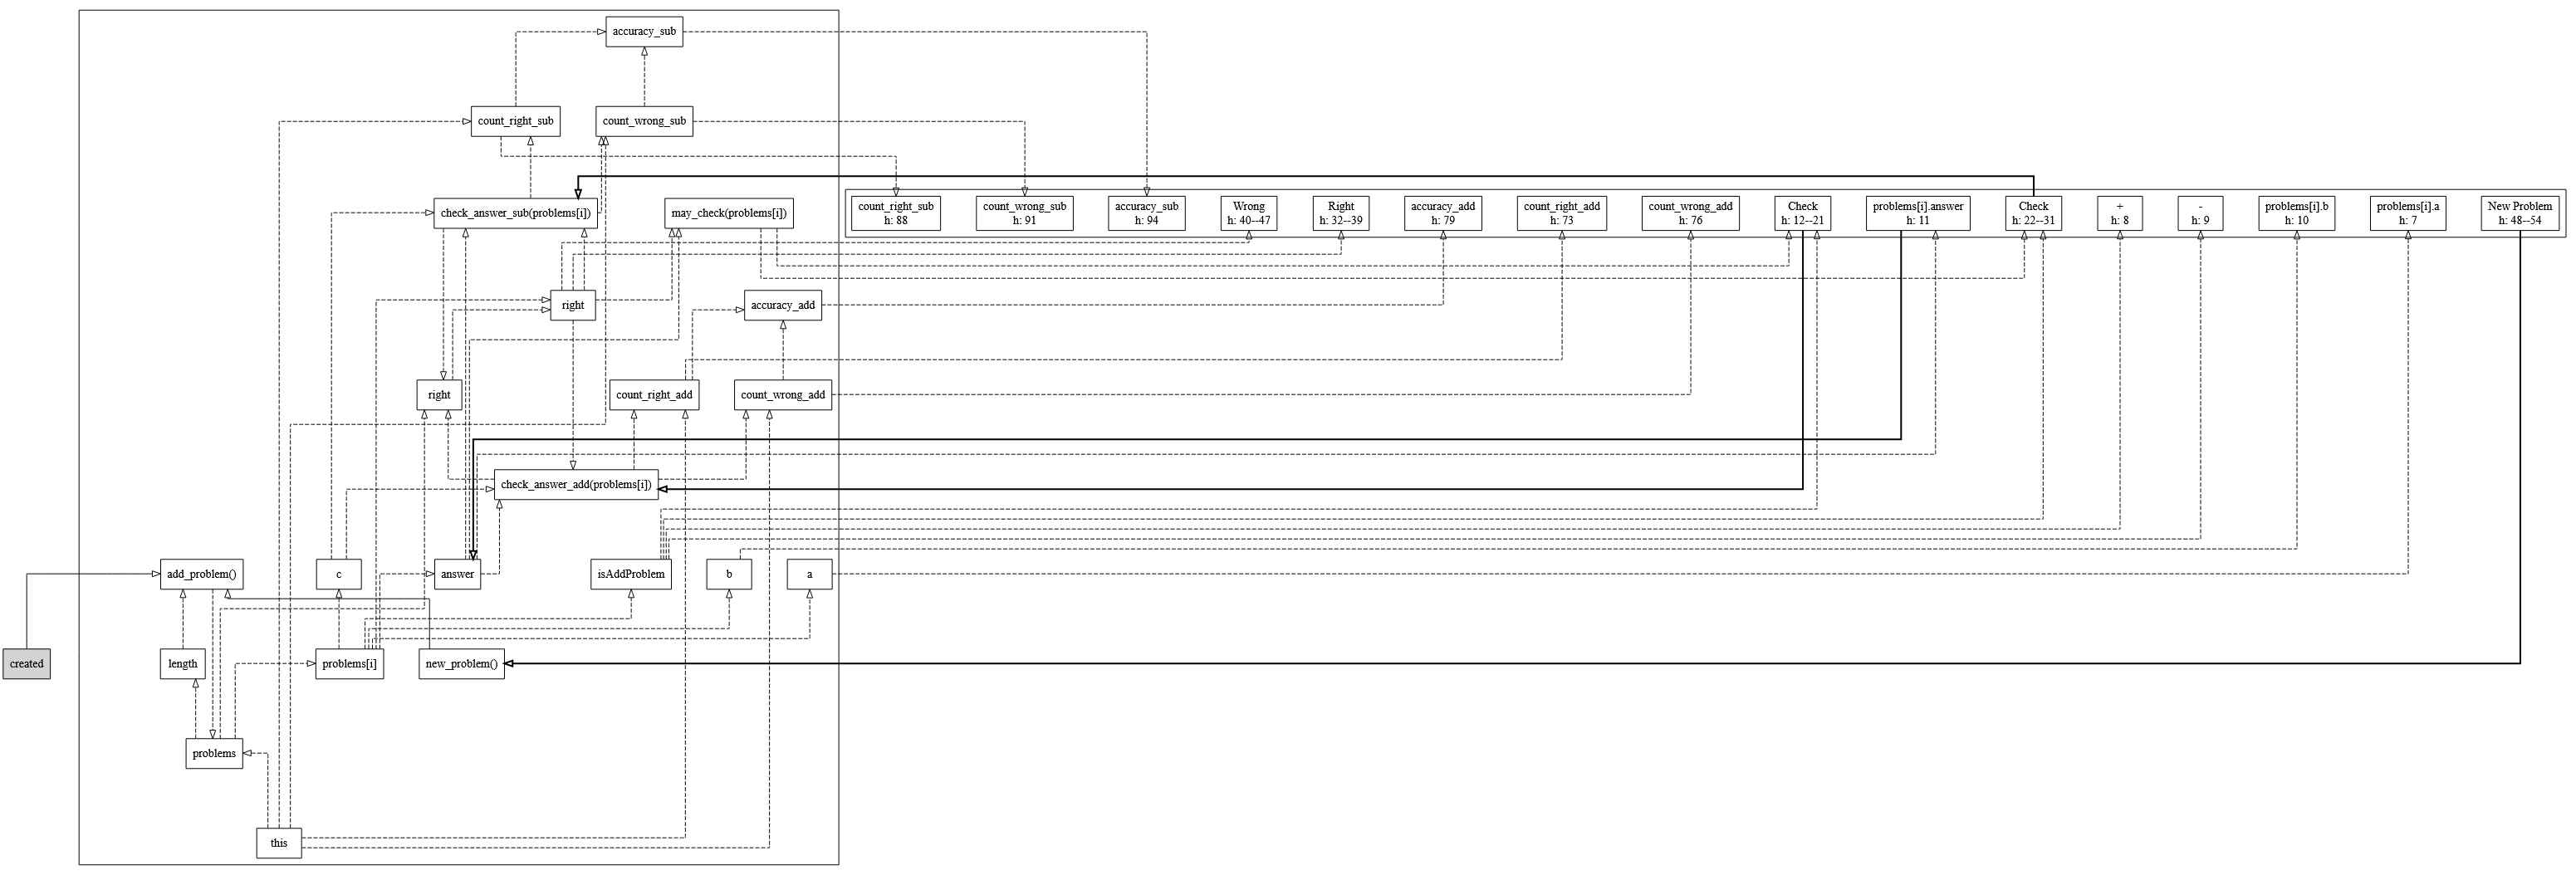
\includegraphics[width=\textwidth]{images/diagram_list_add_sub.png}
     \caption{Generated interaction diagram for Math for Kids including subtraction in Vue.js}
     \label{fig:diagram_list_complex}
\end{figure}



%TODO double check scenarios generated


\section{Menu with daily meal - Lists and Objects}
Another simple example \gls{spa} with the aim of evaluating the capabilities of the application when dealing with lists and complex objects was devised and can be seen in \ref{fig:eval_image_meal}. It shows a which displays a minimalistic menu for a restaurant with a meal of the day. The full source code for it can be found in \ref{appendix:daily_menu_source_code}.

The daily meal and its price is changed every day via a button click, and alternates between the first two items. The third item, steak, is never the daily meal. There is also an option to discount the price of all items. With stakes being the restaurant's special, there is an additional advertisement label them.
\begin{figure}[H]
    \centering
    \begin{subfigure}[t]{0.45\textwidth}
         \centering
         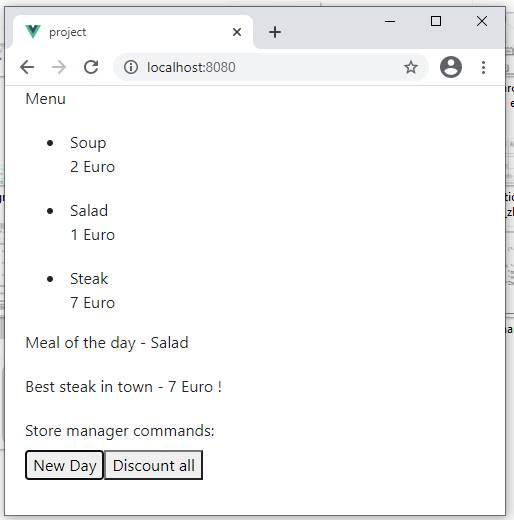
\includegraphics[width=0.45\textwidth]{images/meal_1.png}
         \caption{The current meal of the day is salad.}
    \end{subfigure}\hfill%
    \begin{subfigure}[t]{0.45\textwidth}
        \centering
        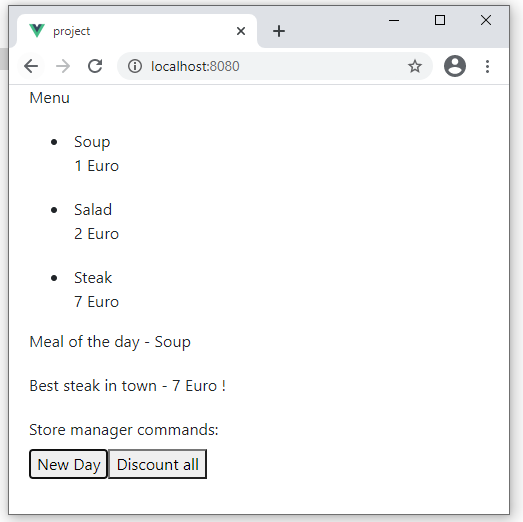
\includegraphics[width=0.45\textwidth]{images/meal_2.png}
        \caption{The 'new day' button has been clicked and the daily meal now changed to soup.}
    \end{subfigure}\hfill%
    \begin{subfigure}[t]{0.45\textwidth}
        \centering
        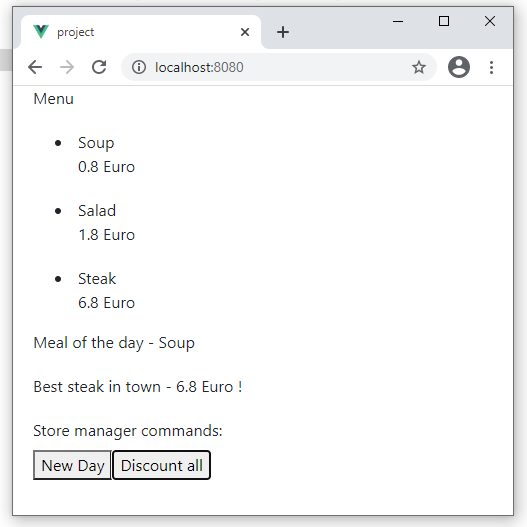
\includegraphics[width=0.45\textwidth]{images/meal_3.png}
        \caption{Discount was clicked and the price of all items got updated.}
    \end{subfigure}
    \caption{The menu with daily meal application }
    \label{fig:eval_image_meal}
\end{figure}

Fig. \ref{fig:diagram_meal_list_properties} shows the interaction diagram for the application. The resulting interactions can be seen in \ref{eval:reactions_meal} and scenarios of up to 4 steps are shown in \ref{eval:scenarios_meal}.
\label{eval:reactions_meal}
\begin{lstlisting}[language=JavaScriptPlain]
l(New Day) -> Price, Meal of the day -
l(Discount all) -> Best steak in town -, Price
l(created) -> meals[i].name, Price, Best steak in town -, Meal of the day -
\end{lstlisting}

\label{eval:scenarios_meal}
\begin{lstlisting}[language=JavaScript,   basicstyle=\fontsize{9}{9}\selectfont\ttfamily]
Scenario: ['created']
	When 'created'
	Then 'meals[i].name'
	And 'Price'
	And 'Best steak in town -'
	And 'Meal of the day -'

Scenario: ['created', 'New Day']
	Given 'created'
	When 'New Day'
	Then 'Price'
	And 'Meal of the day -'

Scenario: ['created', 'Discount all']
	Given 'created'
	When 'Discount all'
	Then 'Best steak in town -'
	And 'Price'
\end{lstlisting}

The \code{New Day} button changes the \code{Meal of the day} and some/all of the \code{Price} list HTML tags. Note that only the price of each meal is changed, the \code{meals[i].name} HTML tags remain the same. \code{Best steak in town} is also not updated, since steak, the last element, is the daily meal. 

Clicking on \code{Discount all} does indeed change both \code{Best steak in town} and some/all \code{Price} HTML tags, since everything is discounted.

\newpage
\begin{figure}[H]
    \centering
    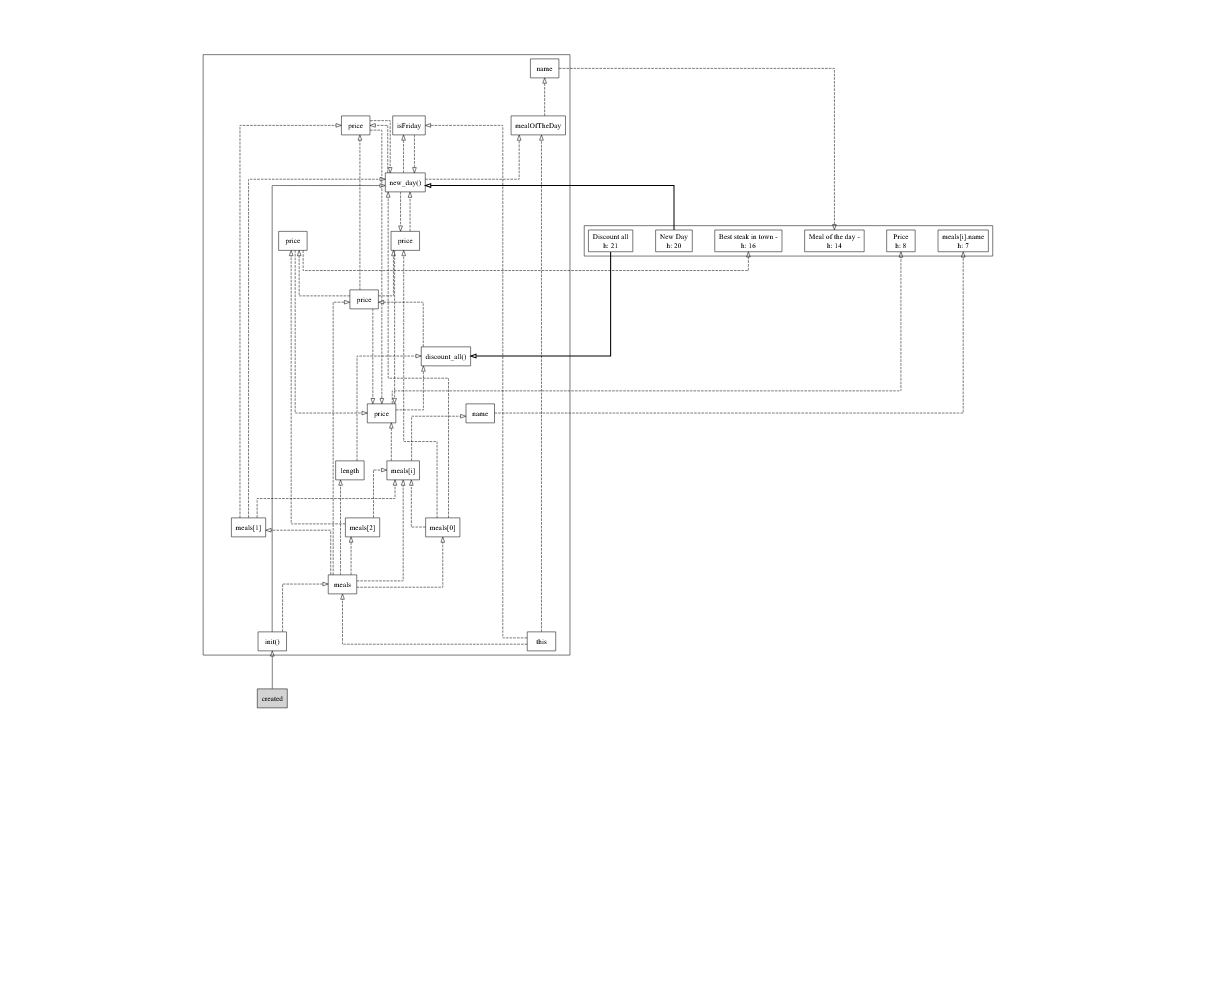
\includegraphics[width=\textwidth]{images/diagram_meal.png}
     \caption{Generated interaction diagram for Menu with daily meal}
     \label{fig:diagram_meal_list_properties}
\end{figure}
